%%%%%%%%%%%%%%%%%%%%%%%%%%%%%%%%%%%%%%%%%%%%%%%%%%%%%%%%%%%%%%%%%%%%%%%%%%%%%
% 13/06/2016
% edited by Isadora Sophia
%
% Feel free to use (copy) the structure (latex formatting source code)
% but not the content of this document.
%
%%%%%%%%%%%%%%%%%%%%%%%%%%%%%%%%%%%%%%%%%%%%%%%%%%%%%%%%%%%%%%%%%%%%%%%%%%%%%

\documentclass[compress, seagull]{beamer}

\mode<presentation>

\usetheme{Warsaw}
% other themes: AnnArbor, Antibes, Bergen, Berkeley, Berlin, Boadilla, boxes, CambridgeUS, Copenhagen, Darmstadt, default, Dresden, Frankfurt, Goettingen,
% Hannover, Ilmenau, JuanLesPins, Luebeck, Madrid, Maloe, Marburg, Montpellier, PaloAlto, Pittsburg, Rochester, Singapore, Szeged, classic

%\usecolortheme{lily}
% color themes: albatross, beaver, beetle, crane, default, dolphin, dov, fly, lily, orchid, rose, seagull, seahorse, sidebartab, structure, whale, wolverine

%\usefonttheme{serif}
% font themes: default, professionalfonts, serif, structurebold, structureitalicserif, structuresmallcapsserif

% pdf is displayed in full screen mode automatically
%\hypersetup{pdfpagemode=FullScreen}

% define your own colours:
\definecolor{Red}{rgb}{1,0,0}
\definecolor{Blue}{rgb}{0,0,1}
\definecolor{Green}{rgb}{0,1,0}
\definecolor{magenta}{rgb}{1,0,.6}
\definecolor{lightblue}{rgb}{0,.5,1}
\definecolor{lightpurple}{rgb}{.6,.4,1}
\definecolor{gold}{rgb}{.6,.5,0}
\definecolor{orange}{rgb}{1,0.4,0}
\definecolor{hotpink}{rgb}{1,0,0.5}
\definecolor{newcolor2}{rgb}{.5,.3,.5}
\definecolor{newcolor}{rgb}{0,.3,1}
\definecolor{newcolor3}{rgb}{1,0,.35}
\definecolor{darkgreen1}{rgb}{0, .35, 0}
\definecolor{darkgreen}{rgb}{0, .6, 0}
\definecolor{darkred}{rgb}{.75,0,0}

\xdefinecolor{olive}{cmyk}{0.64,0,0.95,0.4}
\xdefinecolor{purpleish}{cmyk}{0.75,0.75,0,0}

\usepackage[utf8]{inputenc}

\fboxsep=10mm%padding thickness
\fboxrule=0pt%border thickness

% \usepackage{beamerinnertheme_______}
% inner themes include circles, default, inmargin, rectangles, rounded

%\usepackage{beamerouterthemesmoothbars}
% outer themes include default, infolines, miniframes, shadow, sidebar, smoothbars, smoothtree, split, tree

\useoutertheme[subsection=false]{smoothbars}

% to have the same footer on all slides
%\setbeamertemplate{footline}[text line]{xxx xxx xxx}
%\setbeamertemplate{footline}[text line]{} % or empty footer

\usepackage{verbatim}

% include packages
\usepackage{subfigure}
\usepackage{amsmath}
\usepackage{epsfig}
\usepackage{graphicx}
\usepackage[all,knot]{xy}
\xyoption{arc}
\usepackage{url}
\usepackage{multimedia}
\usepackage{hyperref}
\usepackage{setspace}

\title{Projeto prático}
\subtitle{Implementação da tela azul (Blue Screen of Death) em Linux}
\author{Isadora, Matheus Mortatti, Maurício Lorenzetti e Vitor Alves}
\institute{{\tiny professora}\\ \vspace{.10cm}Islene Calciolari Garcia}
\date{\scriptsize MC504 - Sistemas Operacionais, Unicamp\\ \vspace{.10cm}14 de Junho, 2016}

\begin{document}

\frame{
	\titlepage
}

\section[Agenda]{}
\frame{\tableofcontents}

\section{Ideia}
    %% subsection
    \subsection{Objetivo}
    \frame{\frametitle{Objetivo}

    O objetivo inicial do projeto se baseava na implementação da \textbf{Blue Screen of Death}.

    \vspace{0.25cm}
    \begin{enumerate}
        \item Usuário entra normalmente em seu sistema em Linux. \pause
        \vspace{0.25cm}
        \item O sistema aciona um kernel panic, devido a alguma falha. \pause
        \vspace{0.25cm}
        \item Uma tela azul é instanciada, com informações de DEBUG sobre as possíveis causas do kernel panic.
    \end{enumerate}
    }

    \frame{\frametitle{Exemplo}
        \begin{center}
            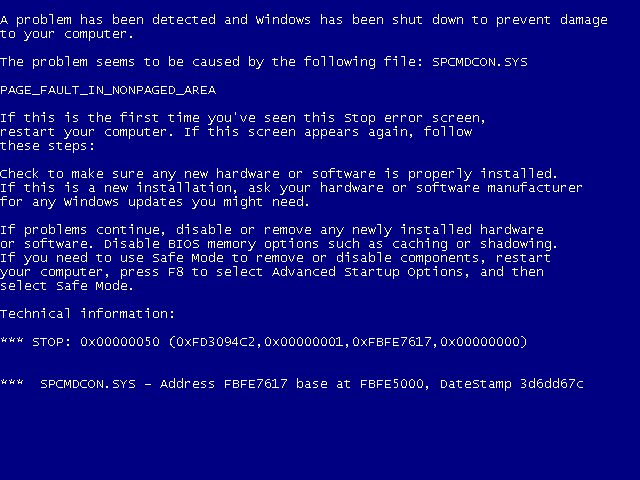
\includegraphics[width=3in, border=false, center]{figures/BSOD}
        \end{center}
    }

    %% subsection
    \subsection{Estratégias}
    \frame{\frametitle{Estratégias}

    Foram estabelecidas diferentes estratégias de soluções para a implementação do projeto.

    \begin{enumerate}
    \item Instanciar uma imagem na tela;
    \vspace{0.25cm}
    \item Imprimir o texto de DEBUG;
    \vspace{0.25cm}
    \item Adicionar features, como áudio, etc.
    \end{enumerate}
    }

\section{Implementação}
    %% subsection
    \subsection{Instanciar imagem na tela}
    \frame{\frametitle{Instanciar imagem na tela}
    \begin{itemize}
    \item Foram utilizados códigos de \texttt{driver/video} como referência para implementação; \pause
    \item Códigos voltados para graphics support; \pause
    \item Exemplos instanciavam logos na tela a partir de imagens \texttt{.ppm}; \pause
    \item Problemas encontrados:
        \begin{itemize}
        \item Instanciação de imagem na tela requer locks e permissões;
        \item Dependente do tipo de display (VGA, HDMI...);
        \item Permissões são restritas devido ao kernel panic;
        \item Uma escrita arbitrária (não autorizada) no kernel leva ao caos!
        \end{itemize}
    \end{itemize}
    }

    \frame{\frametitle{Exemplo de imagem}
        \begin{itemize}
            \item Imagem utilizada para renderização pelo driver:
        \end{itemize}

        \begin{center}
            
\includegraphics[width=1.5in, border=false, center]{figures/logo.png}
        \end{center}
    }

    %% subsection
    \subsection{Impressão de texto}
    \frame{\frametitle{Testes para impressão de texto}
    \begin{itemize}
    \item Tentativas de impressão de texto a partir do acesso da região de memória do ponteiro de \textit{Monochrome Text mode}, ie. \texttt{0xB0000}. \pause
    \item Entretanto, são necessárias permissões para acessar essa região de memória!
        \begin{itemize}
            \item Kernel panic gerava outro kernel panic que gerava outro kernel panic e, por medida de segurança, o sistema reiniciava.
        \end{itemize} \pause
    \item Investigação de métodos de \texttt{drivers/tty}, text-only console (\textbf{T}ele\textbf{TY}pewriter), para impressão na tela; \pause
    \item Encontrada função \texttt{printk}, funcional em kernel panic.
    \end{itemize}
    }

    \frame{\frametitle{Solução com a função printk}
    \begin{itemize}
    \item Problema não estava resolvido. Output precisa ser \textbf{colorido}. \pause
    \item Função \texttt{printk} não suporta customização de cores, como a função \texttt{printf}.
    \end{itemize}
    }

    \frame{\frametitle{Arquivo vt.c}
    \begin{itemize}
        \item Lida com output no \texttt{tty}, text console. \pause
        \item Possui poucas funções visíveis para códigos do kernel.
            \begin{itemize}
                \item Implementada nova função e adicionada no arquivo \texttt{include/vt.h}.
            \end{itemize}
    \end{itemize}

    \begin{center}
        \texttt{extern void vc\_set\_color(int* t\_r);}
    \end{center}
    }

    \frame[containsverbatim]{\frametitle{Arquivo vt.c}
    \begin{verbatim}
/* *
 * Helper function! Reset colors on the current VC
 *   t_r: set as total number of rows of current vc
 * */
void vc_set_color(int* t_r)
{
    struct vc_data* vc = vc_cons[fg_console].d;

    vc->vc_color = blue_screen;

    update_attr(vc);

    *t_r = vc->vc_rows;
}
    \end{verbatim}
    }

    \frame{\frametitle{Máscara de cores}
        \begin{center}
        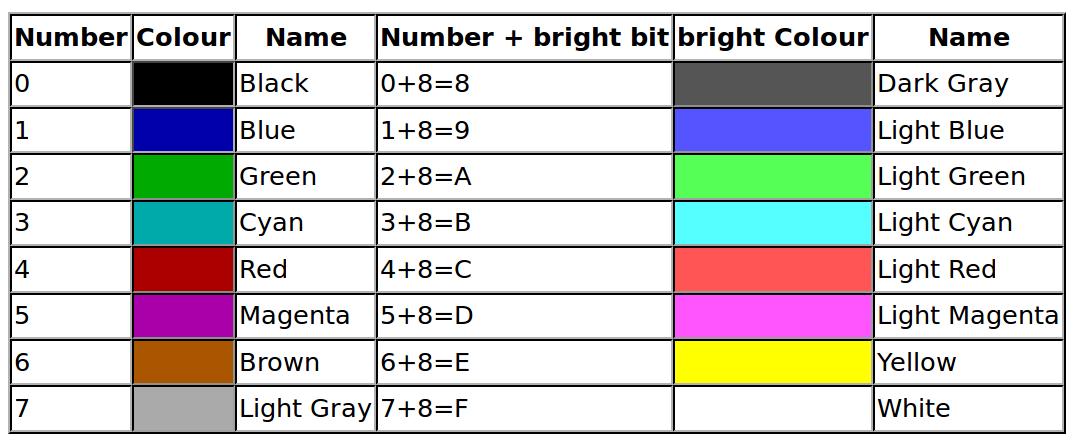
\includegraphics[width=3in, border=false, center]{figures/colors.png}
        \end{center}
    }

    \frame{\frametitle{BSOD.c}
    \begin{enumerate}
        \item Kernel panic ocorre e chama a função \texttt{void display\_error()}, do arquivo \texttt{BSOD.c}; \pause
        \item Função da mudança de cor do TTY é chamada; \pause
        \item Ambiente é modificado e \texttt{printk} é chamado, com mensagem a ser impressa.
    \end{enumerate}
    }

\section*{}
\frame{\frametitle{Demonstração}
    \begin{center}
        \huge
        \texttt{echo c > /proc/sysrq-trigger}
    \end{center}
}

\end{document} 